\documentclass{article}
\usepackage{graphicx}
\usepackage{pdfpages}

\begin{document}

\title{Extensions of L1 Trend Filtering: Seasonality}
\author{David Johnston}

\maketitle

\begin{abstract}
This paper extends and further elucidates ideas from Kim, Koh \& Boyd for L1 regularized
trend filtering and acts a documentation to a repository of a python
implementation using the cvxopt library which can be found at https://github.com/dave31415/myl1tf
\end{abstract}

\section{The primary and dual quadratic programming problems}

We will start off at Section 5.2 of KKB where they state the quadratic programming problem for L1TF
and also state the dual problem.

\begin{eqnarray}
\mbox{minimize} & \frac{1}{2} ~ || y - x ||_2^2  + \lambda ||z||_1 \\
\mbox{subject to} & z = D x
\end{eqnarray}
The first is an $l_2$ norm and the second an $l_1$ norm. The Lagrangian, with a dual variable $\nu \in \mathbf{R}^{n-2}$, is
\[
L(x,z,\nu) =  || y - x ||_2^2  + \lambda ||z||_1 + \nu^T (D x -z)
\]
The dual function is
\[
\mbox{inf}_{x,z} ~ L(x,z,\nu) =
    \left\{
    \begin{array}{ll}
    - \frac{1}{2} ~ \nu^T D D^T \nu + y^T D^T \nu &  - \lambda \mathbf{1} < \nu < \lambda \mathbf{1} \\
  -\infty  & \mbox{otherwise.} \\
  \end{array}
  \right.
\]
and so the dual problem is

\begin{eqnarray}
\mbox{minimize} & \frac{1}{2} ~ \nu^T D D^T \nu - y^T D^T \nu \\
\mbox{subject to} & - \lambda \mathbf{1} < \nu < \lambda \mathbf{1}
\end{eqnarray}

From the solution $\nu^*$ of the dual problem, we can compute the L1TF solution,
\[
x^* = y - D \nu^*
\]

\section{Seasonality}

As suggested by KKB we can adapt this to add a seasonal component.
\begin{eqnarray}
\mbox{minimize} & \frac{1}{2} ~ || y - x -s||_2^2  + \lambda ||z||_1 \\
\mbox{subject to} & z = D x \\
and & \sum_i^P s_i = 0\\
and & s_{i+P} = s_i
\end{eqnarray}

KKB does not go into detail on how to proceed with this and so we will begin here by deriving
the dual problem. We will do this by putting the constraints on $s$ directly into the
equation to be minimized.

To do this, we define $p$ to be the vector of independent variables defining the periodic components.
This vector has dimension $(P-1)$ as the $P$-th, dependent value is $-\sum_{i=1}^{P-1} p_i$ which enforces the constraint that
they sum to zero. This constraint is required if there is to exists a unique solution as otherwise one could add
any constant to $x$ and subtract it from $s$ without changing the model.

We can define $\tilde{p} \in \mathbf{R}^{P}$ as $\tilde{p} = \left( p,-\sum_{i=1}^{P-1} p_i \right) = T p$.
$T$ will be a $P \times (P-1)$ matrix with a $(P-1)$ identity matrix at the top and an extra row consisting of all -1.
The vector $s$ is now just a periodic re-cycling of $\tilde{p}$ which we can represent as s matrix $B$ which is formed by
row-wise stacking some number (ceil(N/P)) of $P \times P$ identity matrices and truncating rows to dimension $N$. So finally
we can write $s = B T p \equiv Q p$. By doing this we can rewrite the optimization problem as

\begin{eqnarray}
\mbox{minimize} & \frac{1}{2} ~ || y - x - Q p||_2^2  + \lambda ||z||_1 \\
\mbox{subject to} & z = D x
\end{eqnarray}
with the $p \in \mathbf{R}^{(P-1)}$ now unconstrained. To improve stabilization and allow more control over $p$, we will add
a $l_2$ regularization constraint and write our problem.
\begin{eqnarray}
\mbox{minimize} & \frac{1}{2} ~ || y - x - Q p||_2^2  + \lambda ||z||_1 + \eta ~ \frac{1}{2} p^Tp\\
\mbox{subject to} & z = D x
\end{eqnarray}

We will now proceed as before and derive the dual problem. To do this we first
write down the Lagrangian
\[
L(x,z,p,\nu,\eta,\lambda) =  || y - x - Q p||_2^2  + \lambda ||z||_1 + \nu^T (D x -z) + \eta ~ \frac{1}{2} p^Tp
\]
and calculate $\mbox{inf}_{x,z,p} L(x,z,p,\nu,\eta,\lambda)$ by setting gradients w.r.t. $x$ and $p$ to zero. The
more subtle minimization w.r.t. $z$ will result in the same constraint in the dual problem as before. The reader
should ensure that they understand how the terms $\lambda ||z||_1 - \nu^T z$ result in the constraint
$- \lambda \mathbf{1} < \nu < \lambda \mathbf{1}$. One can show that outside of this range, the $inf_z$ of this term
is $-\infty$ (at either $z = \pm \infty$) and within is 0 (at $z=0$) and so feasible solutions must lie within.

Setting $\nabla_x L$ =0 yields the equation.
\[
y - x - Qp = D^T \nu
\] or
\[
x = y - Qp - D^T \nu
\]
and $\nabla_p L$ =0 yields
\[
p = \eta^{-1} Q^T D^T \nu
\]
and we can use this last equation for $p$ to solve for $x$ and we can write these solutions as
\begin{eqnarray}
p^* & = &  \eta^{-1} Q^T D^T \nu \\
& and & \nonumber \\
x^* & = & y - D^T \nu - \eta^{-1} Q Q^T D^T \nu
\end{eqnarray}
We then construct the dual problem by plugging these solutions into the Lagrangian and multiplying it by -1
(minimize rather than maximize) and we arrive at
\begin{eqnarray}
\mbox{minimize} & \frac{1}{2} ~ \nu^T A \nu - y^T D^T \nu \\
\mbox{subject to} & - \lambda \mathbf{1} < \nu < \lambda \mathbf{1}
\end{eqnarray}
with
\[
A = D D^T + \eta^{-1} D Q Q^T D^T
\]
We solve this quadratic programming problem as before for $\nu$ and then use the equations above
to calculate $x$ and $p$ from $\nu$. It is apparent that as $\nu \rightarrow \infty$ (seasonality is suppressed),
$p \rightarrow 0$ and we recover the same solution as before for $x$.

\section{Seasonality using $l_1$ regularization}
Finish

\section{Modeling outliers for more robust fits}
Finish

\section{Implementation}
The Githib repository https://github.com/dave31415/myl1tf contains an implementation for this
L1TF modeling with seasonality. This is a fork of the repository
https://github.com/elsonidoq/py-l1tf by Pablo Zivic which implements the
simpler version without seasonality. Both versions are in python and
use the python cvxopt library to solve the quadratic programming problems. Our
version contains some test programs. For example, the following command,
\begin{verbatim}
test_myl1tf.test_l1tf_on_mock_with_period(period=6, eta=1.0,alpha=0.5)
\end{verbatim}
creates a mock data-set, fits the model and displays the following plot.
\begin{figure}
\centering
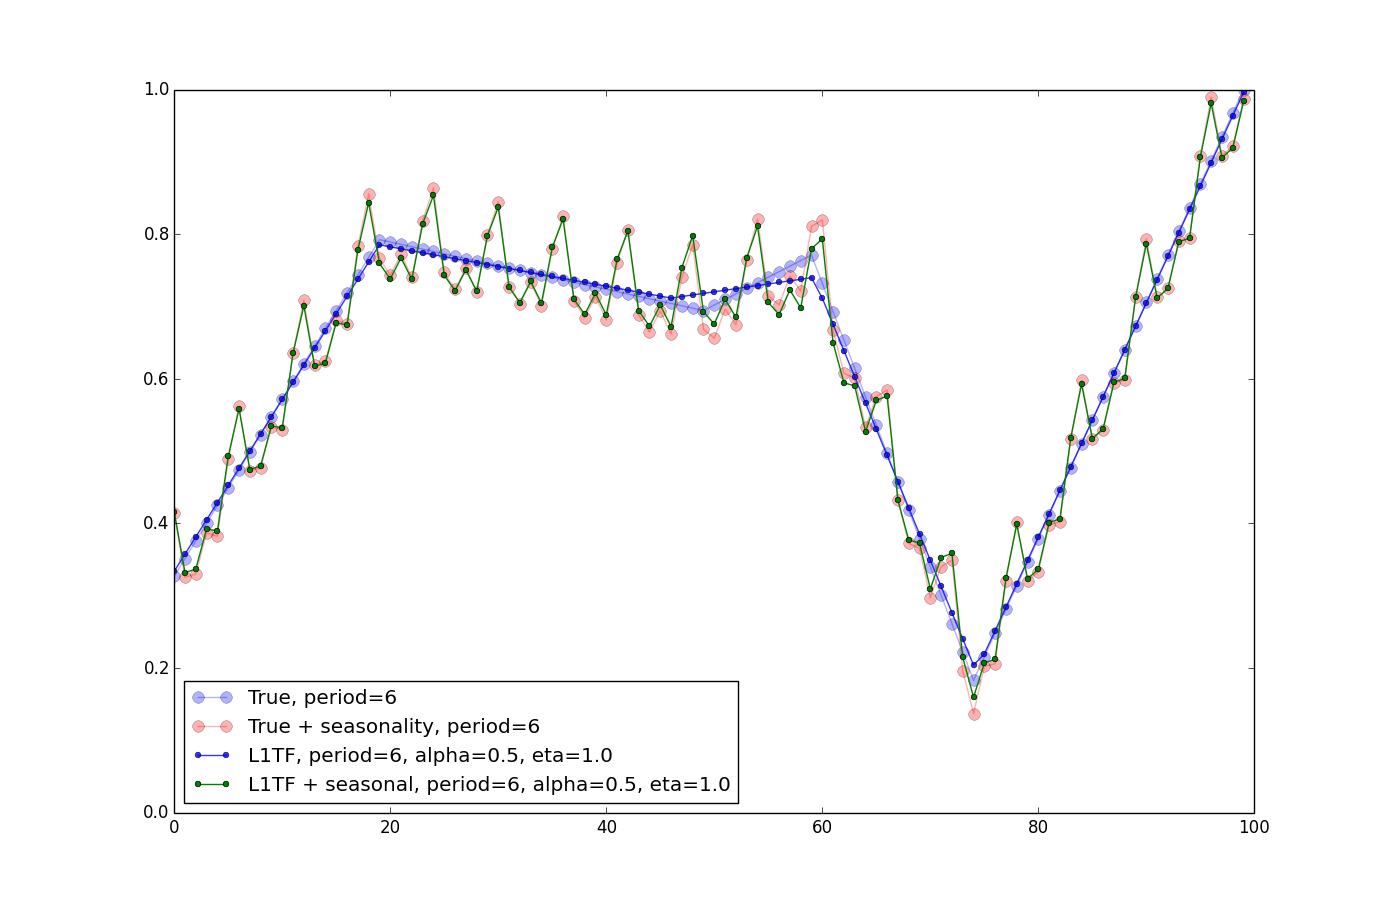
\includegraphics[width=500pt]{example.png}
\end{figure}
(Note alpha = $\lambda$ as lambda is a reserved word in python).

\end{document}

